%%%%%%%%%%%%%%%%%%%%%%%%%%%%%%%%%%%%%%%%%%%%%%%%%%%%%%%%%%%%
\documentclass[a4paper,11pt,oneside]{article}
\usepackage[a4paper,vmargin={1.5cm,1.5cm},width=17cm]{geometry}
\usepackage[style=verbose-inote,doi=false,sortcites=true,block=space,backend=bibtex]{biblatex}
\usepackage[utf8]{inputenc}
\usepackage{textcomp}
\usepackage[english]{babel}
\usepackage{microtype}
\usepackage{lmodern}
\usepackage{graphicx}
\usepackage{fancyhdr}
\usepackage{booktabs}
\usepackage{eurosym}
\usepackage{hyperref}

%%%%%%%%%%%%%%%%%%%%%%%%%%%%%%%%%%%%%%%%%%%%%%%%%%%%%%%%%%%%
%% HEADERS
\setlength{\headheight}{1cm}
\setlength{\headsep}{0.5cm}
\pagestyle{fancyplain}
\fancyhf{}
\lhead{\fancyplain{}{\sc Grant Proposal }}
\rhead{\fancyplain{}{\sc NEXT}}
\cfoot{\thepage}
\renewcommand{\headrulewidth}{0pt} % remove lines
\renewcommand{\footrulewidth}{0pt}

%%%%%%%%%%%%%%%%%%%%%%%%%%%%%%%%%%%%%%%%%%%%%%%%%%%%%%%%%%%%
%% Hack to make math formulas bold in section titles
\makeatletter
\DeclareRobustCommand*{\bfseries}{%
  \not@math@alphabet\bfseries\mathbf
  \fontseries\bfdefault\selectfont
  \boldmath
}
\makeatother

%%%%%%%%%%%%%%%%%%%%%%%%%%%%%%%%%%%%%%%%%%%%%%%%%%%%%%%%%%%%
\def\thesection{\bf \textsf{\alph{section}}}

%\nobibliography{biblio}
%\bibliographystyle{JHEP}

\bibliography{biblio}


%%%%%%%%%%%%%%%%%%%%%%%%%%%%%%%%%%%%%%%%%%%%%%%%%%%%%%%%%%%%
\begin{document}

%% Some useful definitions
% BB
\newcommand{\bb}{\ensuremath{\beta\beta}}
% BB0NU
\newcommand{\bbonu}{\ensuremath{\beta\beta0\nu}}
% BB2NU
\newcommand{\bbtnu}{\ensuremath{\beta\beta2\nu}}
% NME
\newcommand{\Monu}{\ensuremath{\Big|M_{0\nu}\Big|}}
\newcommand{\Mtnu}{\ensuremath{\Big|M_{2\nu}\Big|}}
% PHASE-SPACE FACTOR
\newcommand{\Gonu}{\ensuremath{G_{0\nu}(\Qbb, Z)}}
\newcommand{\Gtnu}{\ensuremath{G_{2\nu}(\Qbb, Z)}}

% mbb
\newcommand{\mbb}{\ensuremath{m_{\beta\beta}}}
\newcommand{\kgy}{\ensuremath{\rm kg \cdot y}}
\newcommand{\ckky}{\ensuremath{\rm counts/(keV \cdot kg \cdot y)}}
\newcommand{\mbba}{\ensuremath{m_{\beta\beta}^a}}
\newcommand{\mbbb}{\ensuremath{m_{\beta\beta}^b}}
\newcommand{\mbbt}{\ensuremath{m_{\beta\beta}^t}}
\newcommand{\nbb}{\ensuremath{N_{\beta\beta^{0\nu}}}}

% Qbb
\newcommand{\Qbb}{\ensuremath{Q_{\beta\beta}}}

% Tonu
\newcommand{\Tonu}{\ensuremath{T_{1/2}^{0\nu}}}

% Tonu
\newcommand{\Ttnu}{\ensuremath{T_{1/2}^{2\nu}}}

% Xe-136
\newcommand{\Xe}{\ensuremath{^{136}}Xe}

% Xe-136
\newcommand{\CS}{\ensuremath{^{137}}Cs}

% Xe-136
\newcommand{\NA}{\ensuremath{^{22}}Na}


% Bi-214
\newcommand{\Bi}{\ensuremath{^{214}}Bi}

% Tl-208
\newcommand{\Tl}{\ensuremath{^{208}}Tl}

% Pb-208
\newcommand{\Pb}{\ensuremath{^{208}}Pb}
% Pb-208
\newcommand{\PBD}{\ensuremath{^{210}}Pb}

% Po-214
\newcommand{\Po}{\ensuremath{^{214}}Po}

% bru
\newcommand{\bru}{cts/(keV$\cdot$kg$\cdot$y)}

% Saltos de carro en tablas
\newcommand{\minitab}[2][l]{\begin{tabular}{#1}#2\end{tabular}}

\newcommand{\thedraft}{0.1.1}% version for referees

\newcommand{\MO}{\ensuremath{{}^{100}{\rm Mo}}}
\newcommand{\SE}{\ensuremath{{}^{82}{\rm Se}}}
\newcommand{\ZR}{\ensuremath{{}^{96}{\rm Zr}}}
\newcommand{\KR}{\ensuremath{{}^{82}{\rm Kr}}}
\newcommand{\ND}{\ensuremath{{}^{150}{\rm Nd}}}
\newcommand{\XE}{\ensuremath{{}^{136}\rm Xe}}
\newcommand{\GE}{\ensuremath{{}^{76}\rm Ge}}
\newcommand{\GES}{\ensuremath{{}^{68}\rm Ge}}
\newcommand{\TE}{\ensuremath{{}^{128}\rm Te}}
\newcommand{\TEX}{\ensuremath{{}^{130}\rm Te}}
\newcommand{\TL}{\ensuremath{{}^{208}\rm{Tl}}}
\newcommand{\CA}{\ensuremath{{}^{48}\rm Ca}}
\newcommand{\CO}{\ensuremath{{}^{60}\rm Co}}
\newcommand{\PO}{\ensuremath{{}^{214\rm Po}}}
\newcommand{\U}{\ensuremath{{}^{235}\rm U}}
\newcommand{\CT}{\ensuremath{{}^{10}\rm C}}
\newcommand{\BE}{\ensuremath{{}^{11}\rm Be}}
\newcommand{\BO}{\ensuremath{{}^{8}\rm Be}}
\newcommand{\UDTO}{\ensuremath{{}^{238}\rm U}}
\newcommand{\CD}{\ensuremath{^{116}{\rm Cd}}}
\newcommand{\THO}{\ensuremath{{}^{232}{\rm Th}}}
\newcommand{\BI}{\ensuremath{{}^{214}}Bi}


%% Heading
\begin{center}
{\Large \textsf{Convocatorias 2014}} \\ \vspace{0.3cm}
{\Large  \textsf{Proyectos de I+D ``Excelencia'' y Proyectos de I+D+I ``Retos Investigación"}} \\ 
{\Large \textsf{Dirección General de Investigación Científica y Técnica}} \\
{\Large \textsf{Subdirección General de Proyectos de Investigación }} \\ 
%\vspace{0.5cm}
%{\LARGE \bf \textsf{Construcción puesta a punto y operación del experimento NEXT en el Laboratorio Subterráneo de Canfranc} }\\ 
%\vspace{0.3cm}
%{\LARGE \bf \textsf{Construction, commissioning and operation of the NEXT experiment at the Canfranc Underground Laboratory }}\\ 
\end{center}


\section{\bf \textsf{SUMMARY OF THE PROPOSAL}}

{\sc Coordinator:} Juan José Gómez Cadenas.
\vspace{0.3cm}

{\sc Title of project:} Construction, commissioning, operation and R\&D for the NEXT experiment at the LSC.
\vspace{0.3cm}

{\sc ACRONYM OF THE COORDINATED PROJECT:} NEXT.
\vspace{0.3cm}

{\sc Groups participating in project:} Instituto de Física Corpuscular (IFIC), Universidad Politécnica de Valencia (UPV), Universidad de Santiago (US) \& Centro de Láseres Pulsados (CLPU). 
\vspace{0.3cm}

{\bf SUMMARY OF THE COORDINATED PROJECT:} 
\vspace{0.3cm}

%%

NEXT (Neutrino Experiment with a Xenon TPC) is an experiment to search neutrino less double beta decay processes (\bbonu). The detection of such processes would demonstrate that neutrinos are Majorana particles (that is their own antiparticles) and would have deep consequences in physics and cosmology.  

The isotope chosen by NEXT is  \XE. The collaboration has access to hundred kilograms of xenon enriched at 90\% in \XE, owned by the Underground Laboratory of Canfranc (LSC). The NEXT technology is based in the use of time projection chambers operating at a typical pressure of 15 bar and using electroluminescence to amplify the signal (\HPXE). The main advantages of the experimental technique are: a) excellent energy resolution; b) the ability to reconstruct the trajectory of the two electrons emitted in the decays, a unique feature of the \HPXE\ which further contributes to the suppression of backgrounds; c) scalability to large masses; and d) the possibility to reduce the background to negligible levels thanks to the barium tagging technology (\BATA).

The NEXT roadmap was designed in four stages: i) Demonstration of the \HPXE\ technology with prototypes deploying a mass of natural xenon in the range of 1 kg; ii) Characterisation of the backgrounds to the \bbonu\ signal and measurement of the \bbtnu\ signal with the NEW detector, deploying 12 kg of enriched xenon and operating at the LSC; iii) Search for \bbonu\ decays with the NEXT-100 detector, which escales up the NEW detector by a factor 2:1 in size (8:1 in mass) and deploys, thus, 100 kg of enriched xenon. iv) Search for \bbonu\ decays with the BEXT detector (Barium-tagging Experiment with a Xenon TPC), which will deploy a mass in the ton scale and will introduce the technology of \BATA\ in order to reduce backgrounds to negligible levels.  

The first stage of NEXT has been successfully completed during the period 2009-2013. The prototypes NEXT-DEMO (IFIC) and NEXT-DBDM (Berkeley) were built and operated for more than two years. These apparatus have demonstrated the main features of the technology. The experiment is currently developing its second phase. The NEW detector is being constructed during 2014 and will operate in the LSC during 2015. The funding for the construction and operation of NEW comes from an Advanced Grant (AdG/ERC) granted to the PI of this project in 2013. The NEXT-100 detector will be built and commissioned during 2016 and 2017 and will start data taking in 2018. NEXT-100 could discover \bbonu\ processes if the period of the decay is equal or less than $6 \times 10^{25}$~year. The fourth phase of the experiment (BEXT) could start in 2020. 

NEXT is an international collaboration, lead by spanish groups (the PI of this proposal is the spokesperson of the collaboration) and with a very significant contribution of US groups. The laser technology needed for the BEXT phase is being developed in collaboration with the Spanish Center for Pulsed Lasers (CLPU). 

 This proposal requires {\em co-funding} to complete the phase three of the experiment. Specifically we request: a) funds to co-finance the construction of the NEXT-100 detector (which is being partially payed by the AdG as well as by the international collaboration, primarily US groups); b) funds to co-finance personnel; and c) a modest contribution of the R\&D to develop the \BATA\ technology.   



 \vspace{0.3cm}

{\bf KEYWORDS OF THE COORDINATED PROJECT:} neutrinos, TPC, HPXe, xenon, double beta decay, Canfranc, high pressure electroluminescence, barium-tagging, laser. 

\section{\bf Introduction}
\label{sec.intro}
The goal of this document is to provide a full justification of the costs requested to the 2014 I+D+i program
``Challenges of society''. This document has been prepared as a complement of the ``Scientific report'' (Memoria científica y técnica) submitted to the 2014 I+D+i program
``Challenges of society'' and is not intended to replace it, but to provide further information to the ministry and evaluators. 

The NEXT experiment is organised as an international collaboration, which includes groups from Spain, Portugal, Russia, USA, and Colombia. The spanish groups participating in NEXT are: Instituto de Física Corpuscular (IFIC), a joined center of the University of Valencia (UV) and the Spanish Council for Research (CSIC). The  Polytechnic University of Valencia (UPV). University of Santiago de Compostela (US). Autonomic University of Madrid (UAM); and University of Zaragoza (UZ). 

The leading groups participating in this coordinated project (IFIC, UPV and US) form the core of the collaboration, while the contribution of UZ and UAM is essentially focused in the radio-purity measurements. The spokesperson (and PI of this coordinated project), the technical coordinator, the software coordinator and the leaders of several working  packages are members of IFIC. The coordinators of the electronics, DAQ, and risk management are members of the UPV. The coordinator of calibration and reconstruction is a member of US. The groups participating in this coordinated project invest 100\% of their research time and resources in the NEXT project. The UZ and UAM share their dedication between NEXT and other projects, and have/will present independent grant proposals.

Furthermore, a strong collaboration is currently being formed between NEXT and the Center for Pulsed Lasers (CLPU), to develop the laser technology which could be used to tag the barium ion emitted in the \bb\ decays, resulting (when combined with the excellent energy resolution of NEXT and its topological signature) in a virtually background-free experiment. We are in the process of preparing a ``white paper'' detailing the theoretical grounds and the experimental procedures to address a successful  \BATA\ program. 

This report is organised as follows. Section \ref{sec.retos} explains the reasons why we believe that the project fits well into the program ``Challenges of society". Section \ref{sec.next} describes the bulk of the project (construction, commissioning and operation of the NEXT experiment at the LSC). Section \ref{next.costs} details the costs of the project (including equipment, personnel, travel and others) and also describes the additional funding sources and the co-funding requested to the I+D+i program.  Section \ref{sec.bata} describes the R\&D \BATA\ program in collaboration with CLPU. Section \ref{bata.costs} details the costs of the R\&D and also describes the additional funding sources and the co-funding requested to the I+D+i program.  Summary and conclusions are presented
in section \ref{sec.conclu}.

\section{\bf The NEXT project and the ``Challenges of society'' program }
\label{sec.retos}
%Si la memoria se presenta a la convocatoria de RETOS INVESTIGACIÓN, deberá identificarse el reto cuyo estudio se pretende abordar y la relevancia social o económica prevista.
%
This research project is presented within the program of ``Challenges of society'', specifically, challenge number 6: {\bf Change and social innovation.}

We argue that this project represents a major innovation in the way that particle physics is conducted in Spain, and thus marks a path to a more productive approach to research.

Particle physics is a clear example of the so-called ``big-science'',
characterised by the need for large budgets, big machines (such as particle accelerators) and large staffs (for example, the number of physicists participating in the ATLAS and CMS experiments is of the order of 5,000). The discovery of the Higgs boson is a quintessential of such big science, and clearly exemplifies its pros and cons. The obvious pro is the major scientific achievement that the discovery represents. Such a discovery has required the construction and operation of the LHC, one the most impressive scientific machines ever built by humankind. The gargantuan scale of the effort could only be met by a collective effort centralised in the largest particle physics laboratory in the World, CERN.  

Among the cons of big science are the large budgets that it involves, often invested in purchasing equipment to be installed at CERN (or other laboratories) and in paying scientific staff whose activity also develops at CERN. Such large budgets are often justified in terms of industrial and scientific returns. While those returns certainly exist, it is often not easy to quantify their impact in the countries that finance big science. Scientific authorship is one example. It is difficult to assign credit, in particular to students and young post-docs, when the detector is built and operated by thousands of physicists, all of them signing, normally in alphabetic order, the scientific papers. Furthermore, returns tend to be larger for countries who are already very developed scientifically. Specifically, the positions of leadership in the large CERN experiments, and in the CERN scientific and technical divisions, are dominated by countries like Germany, Switzerland, U.K., France and Italy. Industrial returns also tend to be larger for those countries. Instead, the scientific and industrial returns for Spain are very modest. 

Remarkably, the countries leading the big science at CERN and other laboratories have also developed ``national science'' physics programs. A case of great interest is Italy, a country not very different from Spain, in terms of GDP and social habits. However, the international impact and the returns of physics in Italy is much larger than in Spain. For example, the number of Spanish staff members at CERN is 115, to be compared with 275 corresponding to Italy (which has the second largest staff population, after France, with 1031 and followed by UK, with 223). Adding fellows and associates (that is, temporary CERN contracts), the figures for Spain are 363, to be compared with 1726 for Italy\footnote{\href{http://council.web.cern.ch/council/en/Governance/TREF-PersonnelStatistics2012.pdf}{http://council.web.cern.ch/council/en/Governance/TREF-PersonnelStatistics2012.pdf}}. Several italians have served as CERN general directors, and have led or are leading the major experiments, such as ATLAS and CMS. The next CERN general director (and perhaps the first woman to occupy such position in the history of the lab) may be the ex-spokesperson of ATLAS, the italian physicist Fabiola Gianotti. Moreover, Italy has four Nobel prizes in physics (Marconi, 1909, Fermi, 1938, Segrè 1959, Rubbia 1984), while Spain has none. 

Remarkably Italy also boasts the best underground laboratory of Europe, and one of the best of the world, the LNGS. The lab hosts 20 experiments including three experiments searching for \bbonu\ processes (GERDA, CUORE and COBRA) and two experiments searching for Dark Matter (WARP and EXO). 

Through these experiments, the italian physics attracts external talent (some of the best physicists from Europe and USA participate in experiments at LNGS) and external funding, complements the big science at CERN with physics of a smaller scale concerning human resources and budgets (the \bbonu\ experiments typically include about 50-100 physicists, including Ph.D. students, to be compared with $\sim 3,000$~of ATLAS or CMS, and the budgets are one order of magnitude smaller). However, such ``local'' physics results in discoveries of great scientific impact (such as the discovery of neutrino oscillations, which has been the result of a world-wide effort involving underground laboratories in Italy, USA, Canada, Russia and Japan). It also allows the training of students and post-docs in experiments where young physicists can made a major impact at all levels, ranging from the construction of the detector to the analysis of the data (this is to be contrasted with the large and hyper-specialised efforts at CERN, where students and post-doc are often restricted to very specific areas of the experiment). Last, but not least, such local science has an important impact in the italian industry and in the appreciation of science by the public in general. 

We argue that, in order to balance and optimise the current big-science effort in Spain, it is necessary to develop the physics of the LSC, in analogy to the italian case. NEXT is the flagship experiment of our national laboratory, and has achieved intentional recognition, as demonstrated by the fact that is a recognised CERN experiment and has obtained an AdG/ERC, the first grant of this type in the field of particle physics. 

We, therefore, consider that the NEXT project is a clear example of social innovation, as it has the potential of implementing profound changes in spanish physics. As described in this project, NEXT, through its various stages, can hit a major discovery. It will bring international credit and visibility to our science and to the LSC. And it has an important impact both in local industry (through contracts to many national firms, and development of high technology) and in the public perception of science (thorough a very intense activity in public forums including large-circulation cultural magazines such as JotDown, where the PI of this project directs the science section). 

Furthermore, the on-going collaboration with the CLPU further reinforces the above arguments, since the effort involves now a second national scientific installation. In addition, the \BATA\ program implies a major example of inter disciplinarity, and can result in a number of important technological returns (development of micron laser technology, which can be applied to molecular fluorescence, among other examples).

It is important to remark that, while the usual operation of big-science in Spain implies to finance the participation of our groups in labs like CERN (including the annual CERN quota, the common-fund of the experiments and the contributions to construction and operation of the CERN experiments), the national science that NEXT represents obtains external funding through ERC projects (including the AdG and several H2020 actions currently in progress involving LSC), as well as the contributions of the international collaboration (in particular, in the case of NEXT through the USA groups led by Prof. Dave Nygren, the inventor of the technology in which NEXT is based and a major driving force of the experiment) to detector construction and operation. NEXT also attracts external talent to our country (as the intense collaboration with top USA universities demonstrates). The NEXT group is very international, and several of our post-docs are of have been financed by EC grants (such as the Marie Curie). 

Last but not least, the NEXT experiment, and in particular the collaboration with the CLPU, involves the extensive development of photonics listed as one of the  "Facilitating Essential Technologies".

\section{\bf The NEXT project}
\label{sec.next}

\subsection*{The NEXT experiment and its innovative concepts}

\begin{figure}
\centering
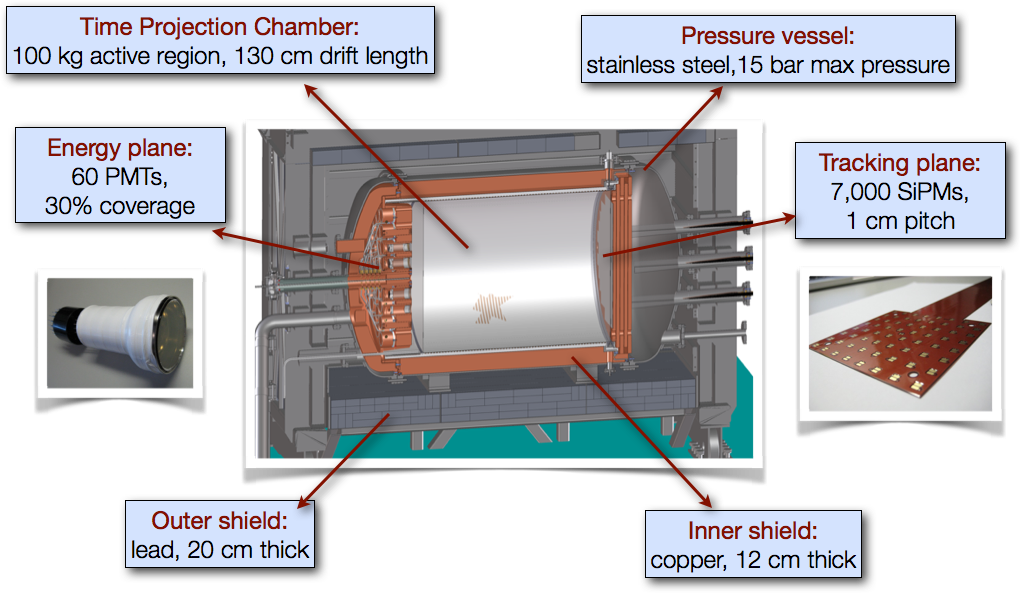
\includegraphics[width=0.9\textwidth]{img/NEXT.png}
\caption{\small A drawing of the NEXT-100 detector showing its main parts.  The pressure vessel (PV),  (130 cm inner diameter, 222 cm length, 1cm thick walls, with a total mass of 1\,200 kg) is made of a radio pure steel-titanium alloy.
The inner copper shield (ICS), is made of ultra-pure copper bars, 12 cm thick, with a total mass of 9\,000 kg.The electrical system includes the field cage, cathode, EL grids and HV penetrators.
The light tube is made of thin teflon sheets coated with TPB (a wavelength shifter). 
The energy plane is made of 60 ultra radio pure PMTs housed in copper enclosures (cans).
The tracking plane is made of SiPMs arranged into dice boards (DB). 
}\label{fig.NEXT100}
\end{figure}

The \emph{Neutrino Experiment with a Xenon TPC} (NEXT)\footnote{\href{http://next.ific.uv.es/}{http://next.ific.uv.es/}} is an experimental program to search for \bbonu\ in \XE\ using  high-pressure xenon gas  time projection chambers (\HPXE). 

The design of the NEXT chambers is optimised for energy resolution by using proportional electroluminescent (EL) amplification of the ionisation signal. The detection process involves using the prompt scintillation light from the gas as start-of-event time, drifting the ionisation charge to the anode by means of an electric field ($\sim0.3$ kV/cm at 15 bar) where secondary EL scintillation will be produced in the region defined by two highly transparent meshes, between which there is a field of $\sim20$ kV/cm at 15 bar. The detection of EL light provides an energy measurement (in the energy plane, made of PMTs, located behind the cathode) as well as providing tracking through its detection a few mm away from production at the anode plane, via a dense array (1 cm pitch) of 1-mm$^{2}$ SiPMs (the \emph{tracking plane}).

The design of the NEXT-100 detector (Figure \ref{fig.NEXT100}) has been described in a \emph{Technical Design Report}.\footcite{Alvarez:2012haa} NEXT-100 has the structure of a Matryoshka (a russian nesting doll). The outermost layer is a shield made of lead, which attenuates the background from the LSC rock by 6 orders of magnitude (e.g., the \TL\ photons are attenuated from $\sim 10^{12}$~per year to $\sim 10^{6}$~per year). The pressure vessel, built out of steel, can hold 150 kg of xenon at 15 bar. Finally, an inner copper shield, 12 cm thick, constitutes the innermost and more radio-clean layer of the Matryoshka. In addition, all NEXT components have been selected and screened for low background. Of particular importance are the PMTs, whose activity is only 0.4 mBq of \BI\ and 0.3 mBq of \TL\ per unit. Our TDR included a detailed background model. A recent paper has validated these results from measurements in a extensive screening campaign carried out in the past year.\footcite{Alvarez:2012as} Currently, most of the major components entering the NEXT detector have been measured, and those numbers are incorporated in our background model. 

\subsection*{NEXT prototypes and the demonstration of the technology}

%%%%%%%%%
%%%%%%%%%
\begin{figure}
\centering
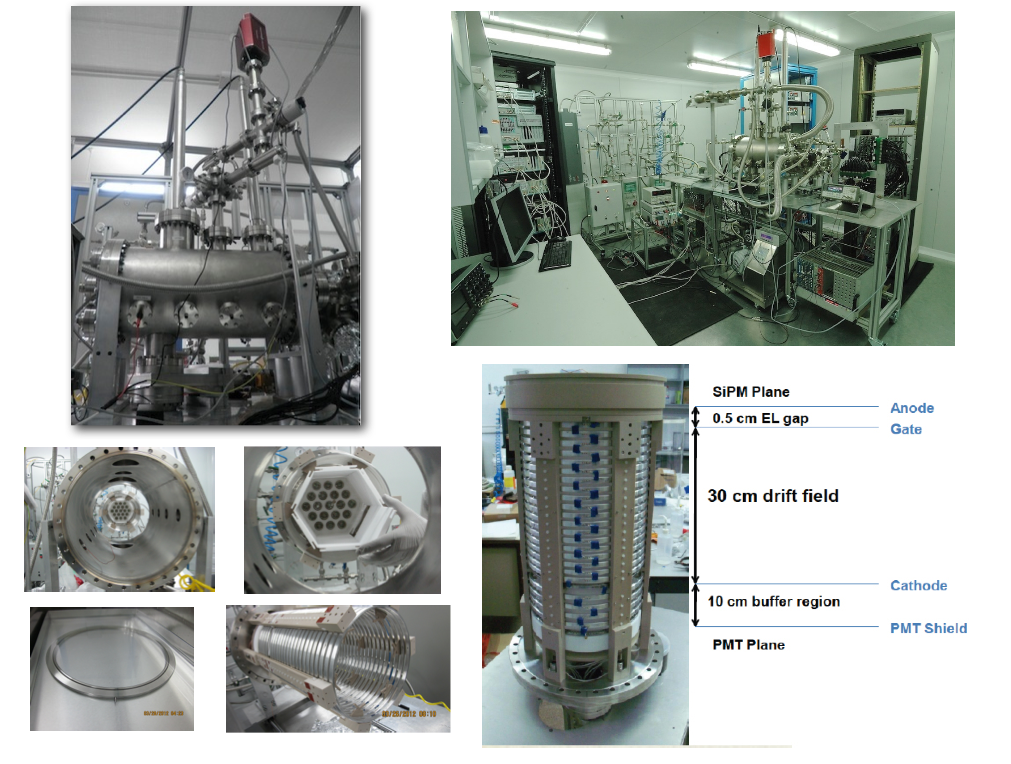
\includegraphics[width=0.7\textwidth]{img/DemoSetup2.png}
\caption{\small The NEXT-DEMO prototype. Top-left: the pressure vessel, showing the HVFT and the mass spectrometer; bottom-left: an expanded view of the detector; (c) Teflon light tube; (d) energy plane, made of pressure resistant Hamamatsu R7378A PMTs; (e) field cage; (f) tracking plane equipped with 300 Hamamatsu MPPCs; top-right: the full setup at IFIC; bottom right: the field cage.} \label{fig.DEMO}
\end{figure}
%%%%%%%%%%

From 2009 to 2013 the NEXT Collaboration has carried out an intense R\&D program (mostly funded by the CONSOLIDER-INGENIO project CUP) that has culminated in the construction, commissioning and operation of the NEXT-DEMO prototype located at IFIC, and the NEXT-DBDM prototype operating at LBNL. The description of these prototypes and the initial results obtained with them have been published\footcite{Lorca:2014sra, Alvarez:2012hh, Alvarez:2012nd, Alvarez:2012hu}.

NEXT-DEMO, shown in figure \ref{fig.DEMO}, is as a large-scale prototype of NEXT-100. The pressure vessel has a length of 60 cm and a diameter of 30 cm. The vessel can withstand a pressure of up to 15 bar. The maximum capacity of the detector is 10 kg but in its current configuration (the fiducial volume is a hexagon of 16 cm diameter and 30 cm length) it holds 4 kg at 15 bar. NEXT-DEMO is  equipped with an energy plane made of 19 Hamamatsu R7378A PMTs and a tracking plane made of 256 Hamamatsu MPPCs. 

The detector has been operating successfully for more than one year and has demonstrated: (a) very good operational stability, with no leaks and very few sparks; (b) good energy resolution ; (c) track reconstruction with PMTs and with SiPMs coated with TPB; (d) excellent electron drift lifetime, of the order of 20 ms. In summary, the operation of NEXT-DEMO has been instrumental in the development of the required knowledge to design and build the NEXT detector.

The NEXT-DBDM prototype is a smaller chamber, with only 8 cm drift, but an aspect ratio (ratio diameter to length) similar to the NEXT detector. The device has been used to perform detailed energy resolution studies. NEXT-DBDM achieves a resolution of 1\% FWHM at 660 keV and 15 bar, which extrapolates to 0.5\% at \Qbb.

\subsubsection*{Topological signature}

%%%%%
\begin{figure}
\centering
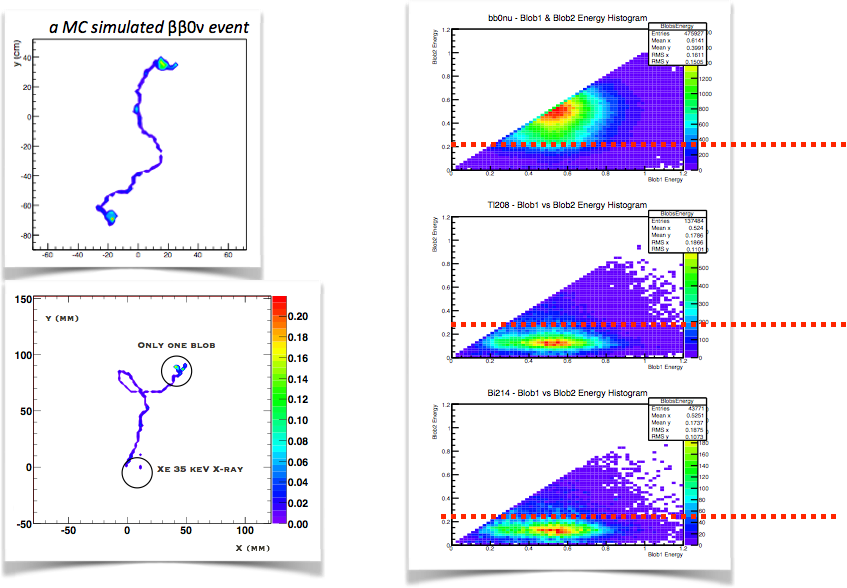
\includegraphics[width=0.9\textwidth]{img/Topology.png}
\caption{\small NEXT has a topological signature, not available in most \bbonu\ detectors. The panel shows the reconstruction of a Monte Carlo signal (topleft) and background (bottomleft) event. The signal has two electrons (two blobs). The background has only one electron (one blob) and the associated emission of a 35 keV X-ray. The color codes energy deposition in the TPC. A scatter plot of the energy of the two blobs shows a clear separation between signal and background regions.}\label{fig.ETRK2}
\end{figure}
%%%%%
	
Double beta decay events leave a distinctive topological signature in HPXe: a continuous track with larger energy depositions (\emph{blobs}) at both ends due to the Bragg-like peaks in the d$E$/d$x$ of the stopping electrons (figure \ref{fig.ETRK2}, topleft). In contrast, background electrons are produced by Compton or photoelectric interactions, and are characterised by a single blob and, often, by a satellite cluster corresponding to the emission of $\sim30$-keV fluorescence x-rays by xenon (figure \ref{fig.ETRK2}, bottomleft).
Reconstruction of this topology using the tracking plane provides a powerful means of background rejection, as can be observed in the figure. In our TDR we chose a conservative cut to separate double--blob from single--blob events which provided a suppression factor of 20 for the background while keeping 80\% of the signal.  

\subsubsection*{Energy resolution}

%%%%%
\begin{figure}
\centering
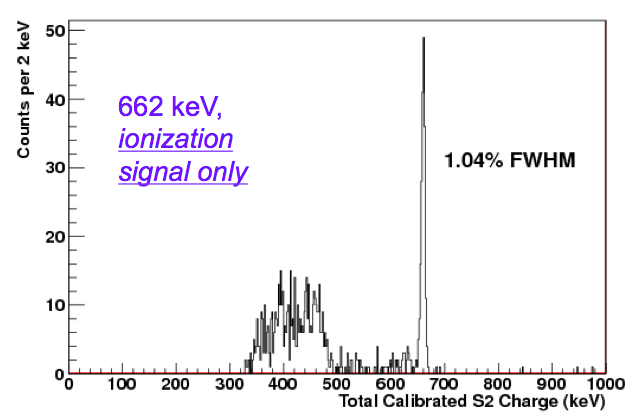
\includegraphics[width=0.6\textwidth]{img/Cs660.png}
\caption{\small The resolution of the photo peak for 662 keV electrons in NEXT-DBDM, at 15 bar is 1\% FWHM (0.5\% FWHM at \Qbb).}\label{fig.ERES}
\end{figure}
%%%%

Figure \ref{fig.ERES} shows the resolution obtained with the NEXT-DBDM apparatus. A resolution of 1\% FWHM with 
662 keV photons has been measured, which extrapolates to 0.5\% FWHM at \Qbb. This result is not far from the expected limit obtained adding in quadrature the different factors that contribute to the resolution (Fano factor, photoelectron statistics and electronic noise). The resolution measured in NEXT-DEMO extrapolates to 0.7\% FWHM. The difference between both prototypes is due to better photoelectron statistics and aspect ratio in DBDM. The results, are, in any case, better than the target of 1\% FWHM described in the TDR.

The status of the NEXT experiment and the results achieved by the prototypes have been described in a recent
paper \footcite{Gomez-Cadenas:2013lta}.

\subsection*{The NEW detector}
\label{sec.new}

%%%%%%%%%%
\begin{figure}
\centering
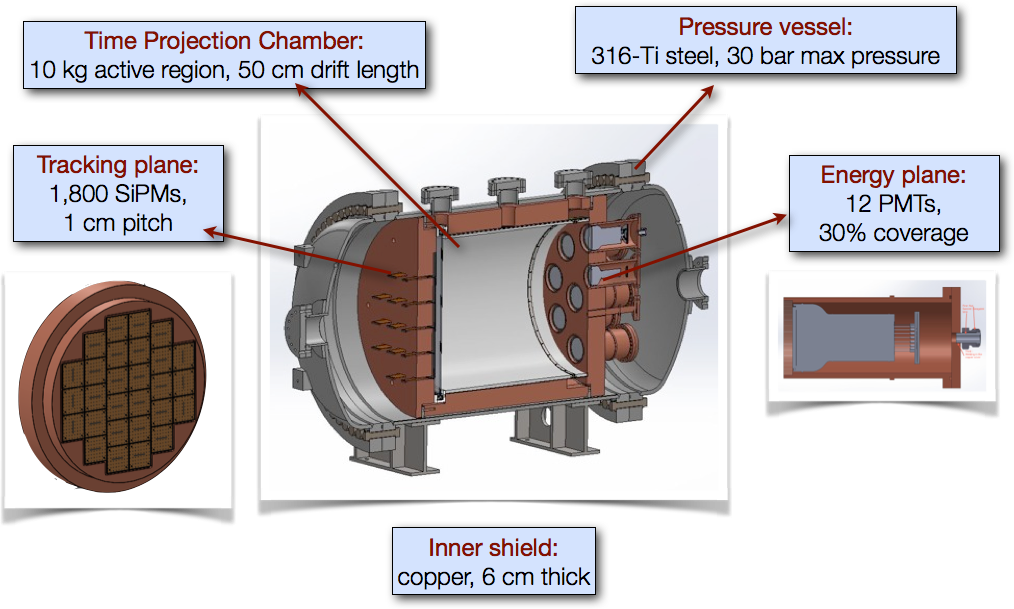
\includegraphics[height=9cm]{img/NEW.png}
\caption{The NEW apparatus.} \label{fig:NEW}
\end{figure} 

The NEW (NEXT-WHITE) apparatus\footnote{The name honours the memory of Professor James White, recently deceased and one of the key scientists of the NEXT Collaboration.}, shown in Figure \ref{fig:NEW} is the first NEXT detector to operate underground. NEW has a triple goal:

\begin{enumerate}
\item {\bf Technology}: it will validate the technological solutions adopted by NEXT-100.
\item {\bf Radiopurity}: it will allow the NEXT collaboration an extra step in the implementation of a radiopure detector.
\item {\bf Physics}: it will demonstrate with measurements of the \BI\ and \TL\ lines, as well as with the measurement of the \bbtnu\ spectrum, the physics capabilities of NEXT-100.
\end{enumerate}

NEW is a scale 1:2 in size (1:8 in mass) of NEXT-100. The energy plane contains 12 radio pure PMTs
of 3 inches diameter, isolated from the gas inside vacuum-tight copper enclosures (we refer to these as PMT cans). The tracking plane technology consists of 30 Kapton Dice Boards (KDB) deploying 1800 SiPMs. The field cage has a diameter of 50 cm and a length of 60 cm. 

\subsection*{Construction schedule}
\label{sec.cons}

The NEW detector is currently (September 2014) under construction. The detector will be assembled at IFIC for functional tests in December 2014, then dismounted and shipped to LSC for exhaustive cleaning (needed to eliminate any possible superficial radioactive contamination) before mounting it again, inside a clean tent in the second quarter (Q2) of 2015. NEW engineering run, needed to certify the technology, will span Q3 and Q4 2015. In 2016, the construction of NEXT-100 will proceed in parallel with the operation of NEW at the LSC. 

The construction of NEXT-100 will benefit of the methodology developed by NEW, since all their systems are scaled-up versions of those in NEW. Taking into account that all sensors are currently acquired (the pressure vessel and infrastructures are also in hand) and adding the fact that the construction procedures needed for NEXT-100 are being developed and extensively tested during NEW construction, the project management plan of the experiment estimates one year for the construction of the large apparatus. NEXT-100 will, therefore, start operations in 2017.

\section{\bf Costs of the NEXT project}
\label{next.costs}

\subsection{Costs of the NEW detector}
Table \ref{tab.new:DET} summarises the total costs of the NEW detector as well as the funding sources. {\bf AdG} refers to the Advanced Grant ERC granted to the PI of this proposal. {\bf CUP} refers to the CONSOLIDER INGENIO grant of which the PI of this proposal is co-coordinator.

Each subsystem is costed in the subsequent tables. Table \ref{tab.new:PV} summarises the costs of the pressure vessel, 
table \ref{tab.new:ICS} the costs of the inner copper shielding,
table \ref{tab.new:EP} the costs of the energy plane,
table \ref{tab.new:TP} the costs of the tracking plane,
table \ref{tab.new:FC} the costs of the field cage,
table \ref{tab.new:FEE} the costs of the front-end electronics and
table \ref{tab.new:DAQ} the costs of the online and data acquisition. The NEW detector has
been fully payed by CUP and AdG grants.

The costs detailed in the tables are very accurate, since most of the components have already been acquired. 
  
\begin{table}[h!]
\begin{center}
\begin{tabular}{|l|c|c|c|}
\hline
 System & Total \euro & CUP & AdG  \\
 \hline
 Pressure vessel 	& 186,668 &	12,6445 &	60,223 \\
Inner copper shield	& 32,670	& 0 &	32,670 \\
Energy plane	& 131,270 &	88,572 &	42,698 \\
Tracking plane	& 82,318 &	0 &	82,318 \\
field cage	& 78,009 &	0 &	78009 \\
FE electronics &	83,661 &	83,661 &	0\\
DAQ and online &	70,391 &	0 &	70,391 \\
 \hline
{\bf Total NEW} &	{\bf 664,989 }& 	298,678 & 	366,311 \\	
 \hline\hline
\end{tabular}  
\caption{Costs of the NEW detector.}
\label{tab.new:DET}
\end{center}
\end{table} 

\begin{table}[h!]
\begin{center}
\begin{tabular}{|l|c|c|}
\hline
 Concept & \euro & Funding Source \\
 \hline
 Tools &	2,144 &	AdG \\
Gaskets & 24,200 &	AdG \\
Carts	& 12,100 &	AdG\\
Machining	 & 21,780 & 	AdG\\
Vessel	& 96,195 &	CUP \\
End-cups	& 15,730 &	CUP \\
Vacuum Pump	& 14,520 & CUP \\
 \hline
{\bf Total}	& {\bf186, 669 }& \\	
Total CUP	& 126,445 & \\	
Total AdG	& 60.223 & \\	
 \hline\hline
\end{tabular}  
\caption{Costs of the NEW pressure vessel.}
\label{tab.new:PV}
\end{center}
\end{table} 

\begin{table}[h!]
\begin{center}
\begin{tabular}{|l|c|c|}
\hline
 Concept & \euro & Funding Source \\
 \hline
 Copper stock &	18,150 &	AdG \\
Machining & 14,520 &	AdG \\
 \hline
{\bf Total} &	{\bf 32, 670} & \\		
Total AdG	& 32,670 & \\	
 \hline\hline
\end{tabular}  
\caption{Costs of the NEW inner copper shield.}
\label{tab.new:ICS}
\end{center}
\end{table} 

\begin{table}[h!]
\begin{center}
\begin{tabular}{|l|c|c|}
\hline
 Concept & \euro & Funding Source \\
 \hline
Support plate	&	14,520 &	CUP \\
PMT cans &	25,250 &	AdG\\
Feedtrhoughs &	14,520 &	AdG \\
R11410-10 (12) &	74,052 &	CUP \\
PMT Bases &		2,928 &	AdG\\
  \hline
{\bf Total}	&	{\bf 131,271}	& \\
Total CUP	&	88,572	&\\
Total AdG	&	42,699 & \\	
 \hline\hline
\end{tabular}  
\caption{Costs of the NEW energy plane.}
\label{tab.new:EP}
\end{center}
\end{table}

\begin{table}[h!]
\begin{center}
\begin{tabular}{|l|c|c|}
\hline
 Concept & \euro & Funding Source \\
 \hline
SiPMs MicroFC-10035-SMT-GP &	29,814 & AdG \\
DICE-Boards SLK-1	&	4,356 & AdG \\
LEDs \& sensors	&	24 & AdG \\
Connectors FX11	&	871 & AdG \\
Inner Cables	&	4,840 & AdG \\
Screws	&	3,630 & AdG \\
Adapter Boards &	4,840 & AdG \\
External Cables &	5,505 & AdG \\
External cables shielding	&	847,00 & AdG \\
SiPM Power Supply Components	& 2,420 & AdG \\
SiPM Power Supply Cables	& 7,260 & AdG \\
Support plate  & 12,100 &  AdG \\
 Feedthrough PCB	&	2,178 & AdG \\
Feedthrough mechanics &	 24,200 & AdG \\
  \hline
{\bf Total}	&	{\bf 82.318,24 }	& \\
  Total AdG	&	82.318,24 	& \\
 \hline\hline
\end{tabular}  
\caption{Costs of the NEW tracking plane.}
\label{tab.new:TP}
\end{center}
\end{table} 

\begin{table}[h!]
\begin{center}
\begin{tabular}{|l|c|c|}
\hline
 Concept & \euro & Funding Source \\
 \hline
 Light tube & 12,877 & AdG \\
 Drift resistor chain & 8,258 & AdG \\
 Buffer resistor chain & 4,386 & AdG\\
 Poly body & 19,844 & AdG \\
 Field shaping rings & 4,451 & AdG \\
 Gate prototype & 4,477 & AdG \\
 Gate & 12,705 & AdG \\
 HVFT \& meshes & 11,011 & AdG \\
  \hline
{\bf Total} &	{\bf 78,009}	& \\
  Total AdG	&	78,009	& \\
 \hline\hline
\end{tabular}  
\caption{Costs of the NEW field cage.}
\label{tab.new:FC}
\end{center}
\end{table} 

\begin{table}[h!]
\begin{center}
\begin{tabular}{|l|c|c|}
\hline
 Concept & \euro & Funding Source \\
 \hline
 PMT FEE & 990 & CUP \\
 SiPM FE boards:  components	&	43,337 & CUP \\
SiPM FE boards: PCB manufacturing &	4,374 & CUP \\
SiPM FE boards: prototypes &	2,815 & CUP \\
SiPM FE boards: component mounting &	4,704 & CUP \\
Cables from FE to DAQ interface &	493 & CUP \\
SiPM FE power supplies & 19,766 & CUP \\
19" crates + fan cooling units	& 1,133 & CUP \\
100 ft power supply cable AWG14 &	783 & CUP \\
SiPM FE board design &	5.263 & CUP \\
  \hline
{\bf Total}	&	{\bf 83,6661}	& \\
 Total CUP	&	83,661	& \\
 \hline\hline
\end{tabular}  
\caption{Costs of the NEW front end electronics.}
\label{tab.new:FEE}
\end{center}
\end{table} 

\begin{table}[h!]
\begin{center}
\begin{tabular}{|l|c|c|}
\hline
 Concept & \euro & Funding Source \\
 \hline
FECs + rear module vATCA &	15,730 & AdG \\
FEC v6 TRG module		&	2,420 & AdG \\
ADC Cards vATCA & 	1,542 & AdG \\
Digital Mezzanine vATCA & 1,452 & AdG \\
Chassis vATCA 6-slot	&	10,527 & AdG \\
GbE CAT6 cables		& 145 & AdG \\
Optic SFP Modules - GbE	& 1.319 & AdG \\
GbE CAT6 cables &	1,815 & AdG \\
PCs (LDC/GDC) & 16,940 & AdG \\
Double port 10Gb &	2,831 & AdG \\
SAI	APC	&	9,680 & AdG \\
Swicth 1GbE	& 4,356& AdG \\
Rack SX 24U & 1, 633,50 & AdG \\
  \hline
{\bf Total} &	{\bf 70,391}	& \\
 Total AdG	&	70,391	& \\
 \hline\hline
\end{tabular}  
\caption{Costs of the NEW DAQ.}
\label{tab.new:DAQ}
\end{center}
\end{table} 




\subsection{Costs of the NEXT-100 detector}
Table \ref{tab.n100:DET} summarises the total costs of the Next-100 detector as well as the funding sources. {\bf FIS2014} refers to our proposal of co-funding submitted to the ``Retos de la Sociedad" I+D+i program. {\bf AdG} refers to the Advanced Grant ERC granted to the PI of this proposal. {\bf CUP} refers to the CONSOLIDER INGENIO grant of which the PI of this proposal is co-coordinator. {\bf USA} refers to funds committed by the USA groups.

Each subsystem is costed in the subsequent tables. Table \ref{tab.n100:PV} summarises the costs of the pressure vessel, 
table \ref{tab.n100:ICS} the costs of the inner copper shielding,
table \ref{tab.n100:EP} the costs of the energy plane,
table \ref{tab.n100:TP} the costs of the tracking plane,
table \ref{tab.n100:FC} the costs of the field cage,
table \ref{tab.n100:FEE} the costs of the front-end electronics and
table \ref{tab.n100:DAQ} the costs of the online and data acquisition. The NEW detector has
been fully payed by CUP and AdG grants.

The costs detailed in the tables are  accurate, since the price of most of the components are estimated directly from the costs of the components already purchased for NEW. 
  
\begin{table}[h!]
\begin{center}
\begin{tabular}{|l|c|c|c|c|}
\hline
 Cost &	Total& 	CUP & USA & FIS2014 \\
 \hline
Pressure vessel &	277,332 & 102,850  &	174,482 & 0 \\
Inner copper shield &	187,550 &	0 & 187,550 & 0 \\
Energy plane	& 625,317 &	265,353	&	123,420	&	236,544 \\
Tracking plane	& 287,237 &	0 & 102,487	& 184,750 \\
field cage	& 184,343 &	0	& 0	&	184,343 \\
FE electronics	& 277,870 &	0 &	0 &	277,870 \\
DAQ and online &	142,775 & 	0	& 0	& 142,775 \\
 \hline
{\bf Total NEXT-100} &	{\bf1,982,426 }& 368,203& 	413,457 & 	1,200,766 \\	
 \hline\hline
\end{tabular}  
\caption{Costs of the NEXT-100 detector.}
\label{tab.n100:DET}
\end{center}
\end{table} 

\begin{table}[h!]
\begin{center}
\begin{tabular}{|l|c|c|}
\hline
 Concept & \euro & Funding Source \\
 \hline
Tools &	24,200 & FIS2014 \\
Carts &	 36,300 & FIS2014 \\
Vessel	& 102,850 & CUP \\
Gaskets 	& 27,104 & FIS2014 \\
Main flange &	24,200 & FIS2014 \\
Bolts & 8,470 & FIS2014 \\
Adaptor CF-DN	 &	16,940 & FIS2014 \\
Connexion Gas System	& 18,150 & FIS2014 \\ 
VCR gaskets	& 968 & FIS2014 \\ 
End-Cup & 18,150 & FIS2014 \\ 
\hline
{\bf Total}	& {\bf277,332 } & \\	
Total CUP	& 102,850 & \\	
Total FIS2014	& 174,482 & \\	
 \hline\hline
\end{tabular}  
\caption{Costs of the NEXT-100 pressure vessel.}
\label{tab.n100:PV}
\end{center}
\end{table} 

\begin{table}[h!]
\begin{center}
\begin{tabular}{|l|c|c|}
\hline
 Concept & \euro & Funding Source \\
 \hline
 Copper stock &	158,510 &	USA \\
Machining & 29,040 &	USA \\
 \hline
{\bf Total} &	{\bf 187,550} & \\		
Total USA	& 187,550 & \\
Total FIS2014	& 0 & \\	
 \hline\hline
\end{tabular}  
\caption{Costs of the NEXT-100 inner copper shield.}
\label{tab.n100:ICS}
\end{center}
\end{table} 

\begin{table}[h!]
\begin{center}
\begin{tabular}{|l|c|c|}
\hline
 Concept & \euro & Funding Source \\
 \hline
Support plate	&	58,080 &	FIS2014 \\
PMT cans &	108,216 &	FIS2014 \\
Feedtrhoughs &	60,000 & FIS2014 \\
R11410-10 (12) &	388,773	& CUP+USA \\
PMT Bases &		10,248 &	FIS2014 \\
  \hline
{\bf Total}	&	{\bf 625,317}	& \\
Total CUP	&	265,353	&\\
Total USA	&	123,420 & \\
Total FIS2014	&	236,544 & \\	
 \hline\hline
\end{tabular}  
\caption{Costs of the NEXT-100 energy plane.}
\label{tab.n100:EP}
\end{center}
\end{table}

\begin{table}[h!]
\begin{center}
\begin{tabular}{|l|c|c|}
\hline
 Concept & \euro & Funding Source \\
 \hline
SiPMs MicroFC-10035-SMT-GP & 102,487 & USA \\
DICE-Boards &15,246 & FIS2014 \\
LEDs \& sensors &	85 & FIS2014 \\
Connectors FX11 & 2,439 & FIS2014 \\
Inner Cables & 16,940 & FIS2014 \\
Screws	& 14,520 & FIS2014 \\
Adapter Boards	 &	16,940 & FIS2014 \\
External Cables &	22,022 & FIS2014 \\
External cables & 3,388 & FIS2014 \\
SiPM Power Supply Components & 9,680 & FIS2014 \\
SiPM Power Supply Cables &	14,520 & FIS2014 \\
Plate  TP:  copper stock &  27,830 & FIS2014 \\
Plate  TP:  manufacturing & 18,150 & FIS2014 \\
Plate  TP:  bolts & 	18,150 & FIS2014 \\
Feedthroughs & 4,840 & FIS2014 \\
  \hline
{\bf Total}	&	{\bf 287,237 }	& \\
  Total USA	&	102,487 	& \\
   Total FIS2014	&	184,750 	& \\
 \hline\hline
\end{tabular}  
\caption{Costs of the NEXT-100 tracking plane.}
\label{tab.n100:TP}
\end{center}
\end{table} 

\begin{table}[h!]
\begin{center}
\begin{tabular}{|l|c|c|}
\hline
 Concept & \euro & Funding Source \\
 \hline
 Light tube & 20,570 & FIS2014 \\
 Drift resistor chain & 8,621 & FIS2014 \\
 Buffer resistor chain & 12,856 & FIS2014\\
 Poly body & 44,700 & FIS2014 \\
 Field shaping rings & 17,182 & FIS2014 \\
 Gate &45,980 & FIS2014 \\
 HVFT \& meshes & 34,364 & FIS2014 \\
  \hline
{\bf Total} &	{\bf 184,343}	& \\
  Total FIS2014	&	184,343	& \\
 \hline\hline
\end{tabular}  
\caption{Costs of the NEXT-100 field cage.}
\label{tab.n100:FC}
\end{center}
\end{table} 

\begin{table}[h!]
\begin{center}
\begin{tabular}{|l|c|c|}
\hline
 Concept & \euro & Funding Source \\
 \hline
 PMT FEE & 5130 & FIS2014 \\
 SiPM FE boards: front panels	& 1,332 & FIS2014 \\
SiPM FE boards: components	&	152,266 & FIS2014 \\
SiPM FE boards: PCB manufacturing	&	12,942  & FIS2014 \\
SiPM FE boards:  mounting	&	18,728 & FIS2014 \\
Cat-6 RJ45 cables &	1,731 & FIS2014 \\
SiPM FE power supplies & 73,416 & FIS2014 \\
19" crates  &	5,666 & FIS2014 \\
100 ft power supply cable &	2,663 & FIS2014 \\
Rack19" 42U height x 600 mm deep &	3,993 & FIS2014 \\

  \hline
{\bf Total}	&	{\bf 277,870}	& \\
 Total CUP	&	277,870	& \\
 \hline\hline
\end{tabular}  
\caption{Costs of the NEXT-100 front end electronics.}
\label{tab.n100:FEE}
\end{center}
\end{table} 

\begin{table}[h!]
\begin{center}
\begin{tabular}{|l|c|c|}
\hline
 Concept & \euro & Funding Source \\
 \hline
FECs v6	&	41,140 & FIS2014 \\
ADC Cards	&	5,082 & FIS2014 \\
CDTC16 v2	&	11,858 & FIS2014 \\
Crate Eurocard 19" 	&	363 & FIS2014 \\
Cat-6 RJ45 cables & 266 & FIS2014 \\
Fan cooling units	&	847 & FIS2014 \\
Power supply & 	16,456 & FIS2014 \\
Power supply connectors &	242 & FIS2014 \\
Rack for Eurocard Crate	&	1,210 & FIS2014 \\
Optic SFP Modules &	4,484 & FIS2014 \\
cables from FEC to PC &	617 & FIS2014 \\
PCs (LDC/GDC)	&	33,880 & FIS2014 \\
Double port 10Gb DA/SFP & 6,606 & FIS2014 \\
SAI	APC	 &	12,100 & FIS2014 \\
Swicth 1GbE	& 4,356 & FIS2014 \\
Rack  SX 24U 	&	3,267 & FIS2014 \\						
  \hline
{\bf Total} &	{\bf 142.775,16 €}	& \\
 Total FIS2014	&	142.775,16 €	& \\
 \hline\hline
\end{tabular}  
\caption{Costs of the NEXT-100 DAQ.}
\label{tab.n100:DAQ}
\end{center}
\end{table} 




\subsection{Costs of the NEXT infrastructures}
The operation of NEXT at the LSC requires extensive infrastructures. In addition to the xenon gas, owned by the LSC (100 kg enriched and 100 kg natural), the laboratory has built the working platform, seismic pedestal and lead castle needed to host the experiment. The NEXT experiment provides the gas system needed to recirculate and clean the gas. Such system is expensive, given the safety requirements, and has been purchased with AdG funds. The AdG also provides funds to buy the clean tent, radon suppression and monitoring system and miscellaneous expenses for a total of some
437 k\euro. Importantly, the infrastructures are fully funded with the contributions of the LSC, CUP and AdG. 
Table \ref{tab.n100:INFRA} summarises the total costs of the infrastructures. The costs detailed in the tables are very accurate, since most of the components have already been acquired. 


  
\begin{table}[h!]
\begin{center}
\begin{tabular}{|l|c|c|c|c|}
\hline
 Cost &	Total& 	CUP & AdG &  LSC \\
 \vline
Gas System &	434,177 &	68,970 &	365,207 &	0 \\
Platform and Castle	& 250,600 & 	0	&0 &	250,600 \\
Xenon (100 kg + 100 kg)	1,056,000	& 0 & 0 &	1,056,000 \\
Lead cleaning	& 44,581 &44,581 &	0 & 0 \\
Cleaning equipment	18,150	& 18,150	& 0	& 0	\\
Clean tent	 & 59878	&	0& 59,878 &	0	\\
Radon suppression 	& 5,400 &	0 &	5,400 &	0	\\
Radon monitoring	6,700 &	0	& 6,700	& 0	\\
 \hline
{\bf Total Infrastructures} &	{\bf1,875,486}& 131,701& 437,185 & 1,306,600 \\	
 \hline\hline
\end{tabular}  
\caption{Costs of the NEXT infrastructures at the LSC.}
\label{tab.n100:INFRA}
\end{center}
\end{table} 



\subsection{Costs of computing, calibration and slow controls}
Computing is estimated in 69,521 \euro\ that will be covered by the AdG grant. The costs of the slow control (18,271 \euro) and the calibration (60,700 \euro, cost dominated by the need to purchase special radioactive sources for calibration) are assigned to FIS2014. 

\subsection{Total costs equipment, NEXT construction}
The total costs in equipment of NEXT construction are summarised in table  \ref{tab.TotalE}. They totalise about 4.6 million \euro\ including the xenon gas (1.1 million \euro). The {\bf external} contributions to the project (e.g, the money that does not come from the spanish science system)
add to 1,286,475 \euro\ ,  a figure slightly higher than the co-funding of 1,279,737  \euro\ 
requested in this project. 

\begin{table}[h!]
\begin{center}
\begin{tabular}{|l|c|c|c|c|c|c|}
\hline
Cost	& Total &	CUP &	AdG	& USA &	LSC &	FIS2014 \\
 \hline
& {\bf 4,626,074} &	798,583 & 	897,218 & 	413,457&	1,306,600 & 1,279,738 \\	
 \hline\hline
\end{tabular}  
\caption{Total costs of the NEXT construction (equipment).}
\label{tab.TotalE}
\end{center}
\end{table} 

\subsection{Costs of personnel for NEXT construction}

The construction, commissioning and operation of the NEXT detectors require of a team of specialised physicists and engineers. This team comes from both national and international universities and research institutions. The contributions of the international collaboration, in particular of the USA groups during the period of R\&D and design of NEXT have been very important for the development of the project. Currently, the spanish groups, in particular those participating in this co-ordinated project have absorbed the know-how brought to the collaboration by the crucial contributions of the Berkeley group (prof. David Nygren, the inventor of the TPC technology) and Texas group (the late prof. James White, who was the leading World expert in high pressure gas chambers). 

The CUP grant have made possible the creation of a world class group at IFIC, which includes the PI, the technical coordinator (Dr. Igor Liubarsky, a renewed expert in the field), two R\&C fellows, one of them senior (Dr. Sorel) and one of them junior (Dr. Novella, who starts this year in the group), six post-docs  (Laing, Ferrario, L\'opez-March,  Renner, Martin-Albo and Monrabal) and 4 Ph.D. students, 2 of whom will present their Ph.D. thesis in 2014 or early 2015. Last but not least, the group has formed several engineers. S. C\'arcel is leading the development of mechanics (with the help of technical mechanics engineer A. Mart\'inez) and J. Rodr\'iguez leads the development of electronics (with the help of technical electronics engineer V. Alvarez).

The group at the UPV brings the essential expertise in front-end electronics and data acquisition. The group includes three experienced engineers, all of them professors at the UPV. Last, but not least, prof. J.A. Hernando, from the University of Santiago has taken the important role of calibration and reconstruction coordinator in NEXT. 

We require co-funding to keep essential personnel for the project. A substantial contribution to personnel at IFIC will come from the  AdG grant, which will provide funds for amount of 1,097,258 \euro\ over the period requested for this grant. This will cover the salary of the technical coordinator (Liubarsky) and 4 post-docs. We expect to obtain 4 post-doc years from national and international grants, in particular from the Marie Curie program (these are 2 years positions). Consequently, the IFIC group requires the equivalent to one full post-doc per for years to this grant.  

IFIC also requests funding to keep our 2 senior engineers (C\'arcel and Rodr\'iguez), who are in charge of essential parts of the project and one technical engineer (external funds, from local agencies, such as the Generalitat Valenciana will be sought to fund the second technical engineer in the team). 

The UPV is in charge of the full development of the electronics and brings in essential man power (with permanent positions). The personnel needed is: a technical engineer to help with the development of the front-end electronics, lead by the electronics coordinator of NEXT (prof J. Toledo), and a senior enginner/computer scientist to help with the dual task of DAQ development (task lead for the DAQ coordinator of NEXT, professor R. Esteve) and online computing.  

Last but not least, we request a post-doc to reinforce the group at the University of Santiago. The group is led by prof. J.A. Hernando, a renowned physicist who has made major contributions to neutrino physics and to flavour physics. Hernando is now full time in NEXT and has taken the role of calibration and reconstruction coordinator. A post-doc to help in these tasks, essential for the performance of NEXT is requested. Santiago will seek for local support and international fellowships for a second post-doc.

The NEXT project is extremely well suited as a training ground for students and post-docs. The project involves the construction, commissioning, operation and data analysis of the most advanced HPXe in the World, and the possibility to participate in a major discovery. The teams are very experienced and well organised. At IFIC, four senior physicists (the PI, Dr. Liubarsky, Dr. Sorel and Dr. Novella) are looking forward to advising students. At UPV, students can work with two of the leading experts in front-end electronics and DAQ in the field. At the US, prof. Hernando is already working with two students in calibration and reconstruction.

At the same time, graduate students are very important for the future of the project and for its impact in science and society. Consequently, the groups in this coordinated project require 3 FPI grants, one per group (we will seek for other grants, such as FPU to enrol further graduate students). 

Table \ref{tab.P} summarizes the personnel requested. Table \ref{tab.new:PT} details the standard salaries
payed to post-docs and engineers. Finally, table \ref{tab.new:PC} describes the personnel costs required to this project.

\begin{table}[h!]
\begin{center}
\begin{tabular}{|l|c|c|c|c|}
\hline
Group &	post-docs	& engineers &	technical engineers & FPI\\
 \hline
IFIC &	1 &	2	&1 (3 yr) &	1\\			
UPV	  & 0	&1 &	1 (3 yr)  &	1 \\			
US	& 1 &	0 &	1 (3 yr)  &	 1\\	
CLPU	& 0 &	0 &	1 (3 yr)  &	 1\\			
 \hline
{\bf Total} & 2 & 3 & 4 & 4 \\
 \hline\hline
\end{tabular}  
\caption{Personnel requested.}
\label{tab.P}
\end{center}
\end{table} 

\begin{table}[h!]
\begin{center}
\begin{tabular}{|l|c|c|c|}
\hline
 &	post-docs	& engineers &	technical engineers \\
 \hline
Cost &	40,000 &	40,000	&30,000 \\					
 \hline\hline
\end{tabular}  
\caption{Table of costs per person per year.}
\label{tab.new:PT}
\end{center}
\end{table} 

\begin{table}[h!]
\begin{center}
\begin{tabular}{|l|c|c|c|c|c|}
\hline
Group &	post-docs	& engineers &	technical engineers &  Total \\
 \hline
IFIC	&160,000 &	320,000 &	90,000 & 570,000 \\
UPV	 &	0 & 160,000 &	90,000 &	250,000 \\
US	& 160,000 & 0 & 90,000 &	250,000\\
CLPU & 0 & 0 & 90,000 & 90,000\\
\hline
{\bf Total} & 320,000 & 480,000 & 360,000 & {\bf 1,160,000} \\
 \hline\hline
\end{tabular}  
\caption{Personnel costs.}
\label{tab.new:PC}
\end{center}
\end{table} 

Notice that the total costs requested in this project are slightly below those provided by external fund sources such as the AdG. 


\subsection{Travel to LSC}
The NEW detector will be installed and commissioned at the LSC in mid 2015. In 2016, NEW will operate at the LSC, while the NEXT-100 detector will be constructed at IFIC, UPV and Texas, among other laboratories. In 2017, NEXT-100 will be commissioned at the LSC. Operation will proceed from 2018 onwards.

During commissioning, we foresee the constant presence at the LSC of one of our mechanical engineers and one of our electronics engineer (4 weeks a month).  This is a must, because IFIC and UPV jointly coordinate the mechanics, electronics and computing of NEXT. In the operation periods, when the detector is stable, this presence can be reduced to one week per month. Concerning post-docs, a constant presence of 2 post-docs or students (4 weeks a month) from our groups is needed. In addition, one student or post-doc in charge of the detector shifts is needed. We also foresee the presence of the PI and technical coordinator for about one week per month during the span of the project. 

Notice that the personnel at the LSC provided by the international collaboration will amply match the personnel provided by this project. The USA groups foresee to deploy at least two physicists to the LSC (4 weeks per month). The portuguese groups will deploy at least two more. Personnel from the University of Zaragoza, which is a part of NEXT, will travel frequently to the LSC. 

To minimise costs, we foresee to rent an apartment near Canfranc (probably at Jaca), and to organise travel car-pooling the teams. The daily expenses are computed conservatively (250 \euro\ per week). 

\begin{table}[h!]
\begin{center}
\begin{tabular}{|l|c|c|c|c|}
\hline
Activities at LSC &	2015 &	2016 &	2017 &	2018\\
 \hline	
Construction &	NEW (6 months) &	NEXT-100 & - & - \\ 		
Commissioning	&NEW (6 months) &	- & NEXT-100 & - \\	
Operation	&	- &  NEW & - & NEXT-100 \\ 	
\hline\hline	
\end{tabular}  
\caption{Activities at the LSC}
\label{tab.ActivitiesLSC}
\end{center}
\end{table}
 
\begin{table}[h!]
\begin{center}
\begin{tabular}{|l|c|c|c|c|}
\hline
Personnel at LSC &	2015 &	2016 &	2017 &	2018\\
\hline							
engineers &	2 x 4 w/m per 6 months &	2 x 1 w/m & 2 x 4 w/m per 9 months  &	2 x 1 w/m\\
post-docs/students & 	2 x 4 w/m per 6 months &	2 x 4 w/m & 2 x 4 w/m &	2 x 4 w/m \\
Technical coordinator &	1 x 1 w/m &1 x 1 w/m &1 x 1 w/m &	1 x 1 w/m \\
PI	& 1 x 1 w/m &	1 x 1 w/m &1 x 1 w/m &	1 x 1 w/m\\
Shifters &	1 x 4 w/m per 6 months &	1 x 4 w/m	& 1 x 4 w/m & 1 x 4 w/m \\
\hline\hline
\end{tabular}  
\caption{Personnel at the LSC. w/m means week per month. }
\label{tab.PersonelLSC}
\end{center}
\end{table}

\begin{table}[h!]
\begin{center}
\begin{tabular}{|l|c|c|c|c|}
\hline
Weeks at LSC &	2015 &	2016 &	2017 &	2018\\
\hline							
engineer& 	48 &	24 &	72 &	24 \\
post-docs/students & 	48	& 96 & 	96 &	96\\
Technical coordinator &	6	& 12	 & 12	 & 12\\
PI	& 6	& 12	 & 12	 & 12\\
Shifters &	24 &	48 &	48 &	48\\
\hline
Total &	132	&192 &	240 &	192\\
\hline\hline
\end{tabular}  
\caption{Weeks at the LSC}
\label{tab.WeeksLSC}
\end{center}
\end{table}

\begin{table}[h!]
\begin{center}
\begin{tabular}{|l|c|}
\hline				
Large apartment rental (month) &	1200	\\		
car-pool trip &	150 \\			
number of car-pool trips & 1 per week \\
subsistence/week &	250 \\
\hline \hline	
\end{tabular}  
\caption{Details of costs}
\label{tab.DetailsLSC}
\end{center}
\end{table}	


\begin{table}[h!]
\begin{center}
\begin{tabular}{|l|c|c|c|c|}
\hline	
Concept &	2015 &	2016 &	2017 &	2018\\
\hline						
Apartment	 & 7,200 &	14,400 &	14,400 &14,400 \\
Trips	& 3,600 &	6,000 &	6,000 &	6,000 \\
Subsistance &	33,000 &	48,000	& 60,000 & 48,000 \\
\hline
Total &	43,800 &	68,400 &	80,400 &	68,400 \\				
\hline \hline				
\end{tabular}  
\caption{Costs travel to the LSC.}
\label{tab.CostsLSC}
\end{center}
\end{table}

Tables \ref{tab.ActivitiesLSC}, \ref{tab.PersonelLSC},  
\ref{tab.WeeksLSC}, \ref{tab.DetailsLSC} and  \ref{tab.CostsLSC} detail the calculation of costs. The total travel to LSC foreseen during the span of this project is 261,000 \euro.




\subsection{Costs of construction, personnel and travel to LSC}
\begin{table}[h!]
\begin{center}
\begin{tabular}{|l|c|c|c|c|}
\hline
Subproject &	Construction &	Personnel  &	Travel& Total\\
\hline
COORD (IFIC)	& 859,091 &	600,000 &	181,000 &	1,640,091 \\
ENG (UPV)	& 420,646 &	190,000	& 40,000	& 610,646 \\
CALREC (US)	& 0	& 160,000	 & 40,000	& 200,000 \\
 \hline\hline
\end{tabular}  
\caption{Costs of NEXT construction, personnel and travel to LSC.}
\label{tab.CostsTotal}
\end{center}
\end{table} 

The total costs of construction, personnel and travel to the LSC amounts to 
{\bf 2,450,737 \euro}. The costs are distributed in three subprojects, called COORD (coordination, IFIC), 
ENG (engineering, UPV) and CALREC (calibration and reconstruction, US). The distribution of costs per subproject is detailed in table \ref{tab.CostsTotal}. Notice that the construction funds requested
by IFIC are matched by those provided by the AdG, and the construction funds requested by the 
UPV are matched by those provided by the USA groups. All the personnel funds are matched by 
funds provided by the AdG. The personnel from the co-ordinated project at the LSC will be matched
by personnel from the international collaboration. 

\subsection{Common fund}

The operation and maintenance costs of NEXT will be covered by contributions of all the groups to a common fund (CF). The CF is being implemented in 2015 and will be firm from 2016 onwards. The CF is implemented by charging an annual quota (2,500 \euro) per Ph.D in the group. Table \ref{tab.CFD} gives the distribution of PH.Ds in the collaboration (as of September 2014) and their contribution to the CF. The total is 100 k\euro\ per year, which is the right order of magnitude to cover for common expenses (including supplies, cleaning material, maintenance of subsystems, nitrogen and argon gas, and replacements of expensive supplies such as gaskets) and to afford modest improvements to the systems. 

\begin{table}[h!]
\begin{center}
\begin{tabular}{|l|c|c|c|}
\hline
Group &	number of Ph.D & 	Contribution \\
\hline
IFIC &	10	& 25,000 \\
UPV	& 3 &	7,500 \\
US	& 2	& 5,000 \\
UAM	  & 2 & 	5,000 \\
UNIZAR	& 6	& 15,000 \\
Portugal 	& 6	& 15,000 \\
Russia	& 3	& 7,500 \\
Colombia	& 3	& 7,500 \\
USA	& 5 & 	12,500 \\
\hline
Total & 40& 100,000 \\
 \hline\hline
\end{tabular}  
\caption{Contributions to NEXT common fund.}
\label{tab.CFD}
\end{center}
\end{table} 

In this project we require funds to contribute to the NEXT CF, corresponding to 3 years (2016, 2017 and 2018). The contributions to 2015 can be covered with remaining funds from CUP. The contribution is
37,500 \euro\ per year, thus a total of 112,500 \euro. 
		
\section{\bf The R\&D \BATA\ program}
\label{sec.bata}
The priority of this project is the construction, commissioning and operation of the NEXT experiment. However, the greatest potential of NEXT is, in fact, its capability to become the {\bf leading World experiment} of the field. 

%%%%%%
\begin{figure}
\centering
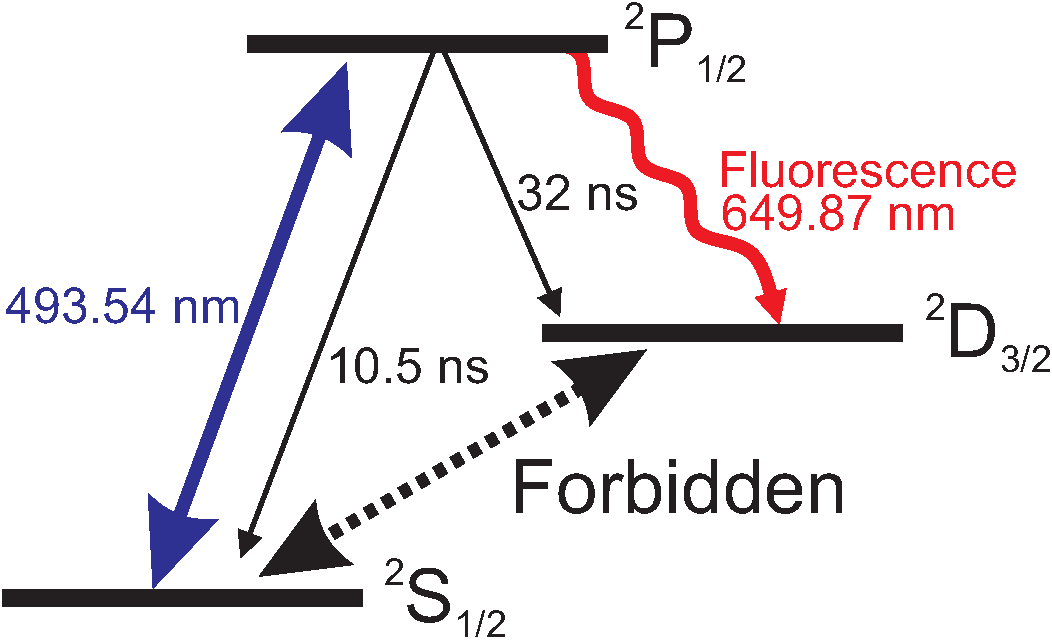
\includegraphics[width=0.5\textwidth]{img/levelscheme.pdf}
\caption{\label{fig.levelscheme} Level scheme for BaTa.} 
\end{figure}
	
%%%%%%

If no discovery is made by the current generation of experiments, the search for \bbonu\ processes will require detectors of larger mass (at least 1 ton), good resolution and extremely low specific background. The \HPXE\ technology has the potential to provide the most sensitive detector in the ton scale, by scaling the detector to a mass in the range of the ton and adding additional handles to further suppress the background. 

One of the most promising possibilities is to develop the technology to unambiguously tag the barium ion produced in the xenon decay, $Xe \rightarrow Ba^{++} + 2 e$. The conceptual idea to tag $Ba^{+}$ is illustrated in Figure \ref{fig.levelscheme2}. A ``blue'' laser of wavelength 493.54 nm excites (``pumps'') the S state, inducing $S \rightarrow P$~transitions, with a lifetime of $\sim$ 10 ns. About 30 \% of the times the \TwoP\ states decay to the state \TwoD, emitting ``red'' (649.86 nm) fluorescence in a characteristic time of 30 ns. The state \TwoD\ is metastable, but a second laser of suitable wavelength (2051.66 nm) can be used to induce the transition to the ground state (this is known as ``deshelving'').  The whole cycle takes less than 50 ns, and therefore several millions of red fluorescence photons can be emitted by a single ion. 

Of course, the practical application of this beautiful conceptual idea is by no means easy, and in fact, it has been shown to be extremely difficult in liquid xenon by the work of the EXO collaboration. However, it may be feasible in an \HPXE\ detector, where a number of fortunate conditions may occur. These conditions are: a) charge reduction of the emitted barium ion, from $Ba^{++}$~to $Ba^{+}$, which can be induced by collisions with xenon atoms, or by the addition of a suitable quencher, such as TEA, as demonstrated by Sinclair et al\footnote{Sinclair.}, b) ``trapping'' of the barium ion ``in situ'' by the surrounding Xe atoms, which result in a very low drift velocity for the ion; c) location of the ion, done by reconstructing the event vertex. 

All the above needs to be demonstrated with a systematic R\&D program, which must also address many other experimental issues such as pressure broadening of the laser, filtering of Rayleigh scattering, etc. Most importantly, such an experimental program must be carried out by an interdisciplinary group, combining the experience in laser spectroscopy and atomic physics, with the experience in \HPXE\ instrumentation.

The on-going collaboration between the IFIC (and other groups of NEXT) and the Center for Pulsed Lasers (CLPU)\footnote{\href{http://www.clpu.es}{http://www.clpu.es}}, a national facility dedicated to ultra-intense lasers research and development has made possible to create precisely the interdisciplinary team needed for a successful R\&D program, which can culminate in a ``Barium-tagging Experiment with a Xenon TPC'' (BEXT). We are currently preparing a white paper which describes the theoretical grounds and details the experimental program to be developed. 

Clearly the construction of a ton-scale \HPXE\ detector implementing a full \BATA\ technology is a very challenging enterprise. On the other hand, we believe that the incremental approach devised by the NEXT collaboration will also work in this case. The construction of the NEW detector is progressing without significant problems thanks to the expertise and know-how gained during DEMO phase, and we expect that NEXT-100 will fully benefit from the experience gained with NEW. Similarly, the \BATA\ technology could be demonstrated in the period of 4 years corresponding to this project,by approaching the problem step by step. 

This is possible only thanks to the collaboration between NEXT and the CLPU.
CLPU is the centre of reference in Spain regarding laser technology, and takes active part in several international and national projects. CLPU enters this co-ordinated project with a full time physicists, who will lead the subproject, Dr. Alicia V. Carpentier who has a well recognised international trajectory in laser-matter interaction. Moreover, CLPU considers this project of high priority and consequently will offer the collaboration of all the scientific department. This consists of a multidisciplinar team with broad experience in laser technology and development, and laser-matter interaction. 

Furthermore, CLPU will support this project with some of the already operating laser systems in its installation. This is extremely important because such systems usually cost of the order of several hundreds of thousand euros which is totally out of the economical scope of this project. The human resources needed to operate the laser systems will be provided by CLPU as well. We will  also like to mention that the small components needed for the construction of the small prototypes will be afforded by the already established NEXT-CLPU collaboration (funds from AdG). In addition, the CLPU and IFIC groups will apply for  \emph{EXPLORA} grants in the next calls.

The different objectives of this subproject are:


\subsection{The \BATA\ program}
The R\&D of the Barium Tagging (\BATA) program includes:

\begin{figure}
\centering
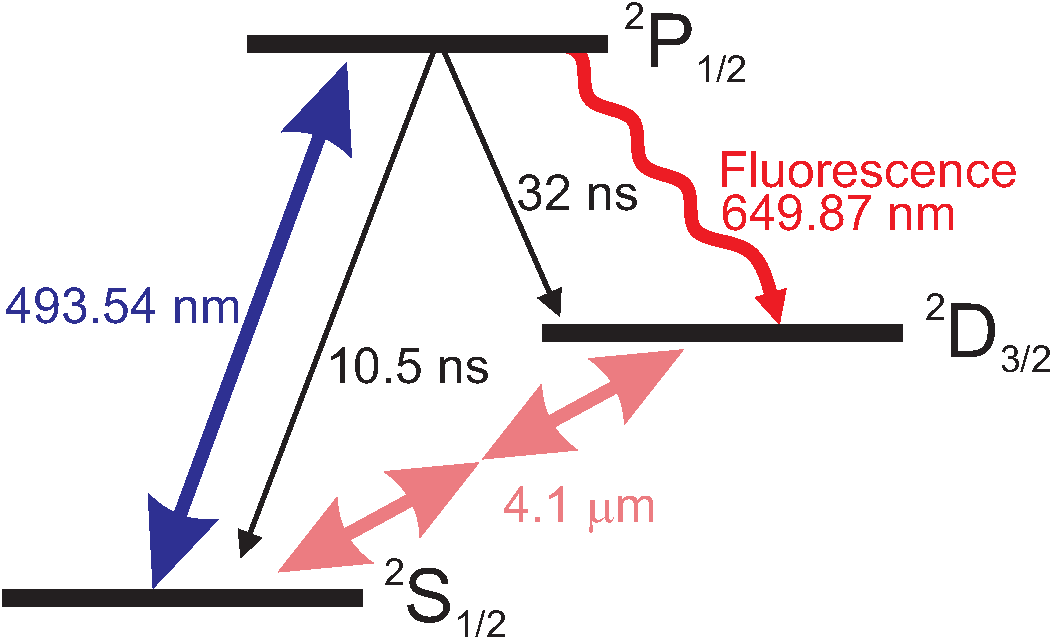
\includegraphics[width=0.5\textwidth]{img/levelscheme2.pdf}
\caption{\label{fig.levelscheme2} Level scheme for BaTa with an infrared deshelving laser.} 
\end{figure}

\begin{itemize}
	\item \textbf{Proof of principle experiment with Ba ions generated by means of an electrical discharge.}
In a first round of experiments we will excite resonantly the S$\leftrightarrow$P transition of Ba$^+$ ions generated by an electrical discharge between two barium electrodes and will collect the fluorescence signal of the P$\rightarrow$D transition (see Figure.\,\ref{fig.levelscheme}). Although this generation method is not ideal because several different species different from Ba ions will be generated, e.g., molecules like BaO or clusters, it does not need a major technological development. It is expected that this initial set of experiments will provide valuable information about the population dynamics in Ba$^+$ ions, and the influence of the different homogenous and in-homogenous broadening mechanisms. It is important to mention that the laser system required for this objective will be provided by the CLPU, and the rest of the material by the ongoing collaboration NEXT-CLPU (e.g., AdG grant).

	\item \textbf{Proof of principle experiment with Ba ions generated by an ion source to be developed.}	
In this objective, in order to get a better approximation of the final conditions of NEXT experiment and with the financial support of a future EXPLORA project, a source of ions will be designed and constructed. This ion source will be based on selective ionisation and mass spectrometry techniques, and it will allow a perfect selection of a target specie. Once the source is ready we will repeat the set of experiments of the previous objective but without any parasitic contribution of unwanted compounds. 
	
	\item \textbf{Proof of principle experiment with Ba ions generated by means of a developed ion source and with a magneto trap.}	
Once the ion source is in operation, in a following objective, we will develop a magneto trap for Ba$^+$  ions. This trap will allow us to have an excellent degree of control over the experimental conditions and to approach the conditions of NEXT. For instance we will carry out different measurements comparing the collected fluorescence signal as a function of the pressure of the Ba$^+$ ions and the pressure of the surrounding environment. These measurements are mandatory because the population dynamics is really sensitive to pressure, i.e., to collisions. 
	
	\item \textbf{Proof of principle experiment with an additional laser for deshelving the D state.}
A possible scenario is that the collisional induced decay between the metastable state D and the ground state S is either not effective or too slow for obtaining an appreciable fluorescence signal. In this situation the population is trapped in the metastable state D  and the fluorescence cycle can not be closed. To avoid this difficulty our approach will be to use a second laser to induce a two photon transition, one photon is forbidden by selection rules, between the states D and S (see Figure.\,\ref{fig.levelscheme2}). This laser must have a wavelength of around 4.1\,$\mu$m which is not easily accesible by commercial laser systems. Our objective is therefore to develop a laser system at this wavelength, and to repeat the experimental matrix defined in previous objectives with two lasers.
	
\end{itemize}

\section{\BATA\ R\&D costs}
\label{bata.costs}

\subsection{R\&D requirements}
The R\&D costs requested to this project are modest. They are:
\begin{enumerate}
\item {\bf A contribution to build an infra-red laser}. The AdG and funds from CLPU cover most of the items needed for the R\&D in 2015 and we fully expect that the EXPLORA project (plus one or more H2020 projects) will cover the R\&D program for the subsequent year. However, a much needed and not fully covered item is a (infra-) red laser of 4.1\,$\mu$m. Such system is needed in our experiments to enhance the transitions between the meta-stable D state in the Ba+ ion and the ground state. On the other hand, it is important to remark that this specific wavelength is not easily accesible by  commercial laser systems, and in fact, there is keen interest in the laser community to develop such laser, due to the fact that this wavelength is not absorbed by the atmosphere and therefore presents many different technological applications. We expect to be able to patent the design and believe it is a clear case of obvious and important industrial return. 
\item {\bf A modest contribution to acquire small equipment and fungible at UPV and US}.
\item {\bf One FPI grant}, to work at the CLPU, in the \BATA\ program. 
\end{enumerate}

\subsection{R\&D costs}
We require a total of 150,000 \euro\ for this program. The bulk of the cost is the development of the infra-red laser (100,000 \euro). To this, we add 25,000 \euro\ for small equipment and fungibles at the US and at the UPV. 

\section{Conclusions}
\label{sec.conclu}

This report summarises the scientific and economic data relevant to the NEXT project, including the R\&D \BATA\ program. The report fully describes the co-funding request to the I+D+i program of ``Challenges of society''. In addition to its scientific excellence, we would like to remark that NEXT is unique in the area of particle physics. As an international collaboration being developed in our national underground laboratory (LSC) and lead by spanish groups, it brings to Spain considerable know-how and external funding. In particular, it is currently the only example of particle-physics experiment in Spain having obtained an advanced grant of the ERC (granted to the spokesperson and PI of this project), 

Of particular interest is also the collaboration with CLPU, which expands the scope of this project to a very interdisciplinar field, including atomic physics and laser-matter interaction. The prospects of industrial returns in the \BATA\ program appear very high, in particular thanks to the development of infra-red laser technology and controlled ions sources, areas with an increasing number of industrial and scientific applications. 

Last but not least, the NEXT experiment, and/or the future BEXT experiment, including the \BATA\ technology have the clear potential of leading a major scientific discovery.

\end{document}

